\documentclass[12pt,a4paper]{article}
\usepackage[utf8]{inputenc}
\usepackage[T1]{fontenc}
\usepackage{amsmath}
\usepackage{amssymb}
\usepackage{graphicx}
\usepackage{hyperref}
\usepackage{geometry}
\usepackage{booktabs}
\usepackage{float}
\usepackage{caption}
\usepackage{subcaption}
\usepackage{helvet}
\renewcommand{\familydefault}{\sfdefault}
\usepackage{enumitem}
\usepackage{bm}

\geometry{margin=1in}

\title{Double Machine Learning for Causal Inference:\\
A Comparative Framework for Model Evaluation, Specification, and Validation in Economics}
\author{}
\date{}

\begin{document}

\maketitle

\section{Introduction: The Econometric Shift from In-Sample Fit to Predictive Performance}

The empirical practice of economics is currently undergoing a structural transformation, driven by the increasing availability of high-dimensional data and the maturation of machine learning (ML) techniques. For decades, the gold standard of causal inference in observational studies---where randomized control trials are infeasible---relied on the linear regression model. Economists have traditionally selected control variables based on a combination of economic theory and intuition, assessing model adequacy through in-sample metrics such as the adjusted $R^2$, F-statistics, and the stability of coefficients across stepwise specifications. However, this classical approach faces severe limitations when the number of potential confounders ($p$) is large relative to the sample size ($n$), or when the functional form of the relationship between confounders and the outcome is highly non-linear and unknown. In these high-dimensional settings, traditional Ordinary Least Squares (OLS) estimation inevitably succumbs to overfitting or omitted variable bias, rendering standard inference invalid.

Double Machine Learning (DML), also known as Doubly Debiased Machine Learning, has emerged as a rigorous methodological solution to this impasse. By integrating flexible ML algorithms---such as Random Forests, Gradient Boosted Trees, Lasso, and Deep Neural Networks---into the causal inference pipeline, DML allows researchers to control for confounding factors in a data-driven manner without specifying a functional form a priori. Yet, for the applied economist accustomed to the interpretability of regression tables, adopting DML requires a fundamental epistemological shift. The focus of model evaluation must move from in-sample goodness-of-fit and parameter significance of control variables to the out-of-sample predictive performance of nuisance parameters.

This report provides an exhaustive examination of the evaluation criteria, diagnostic techniques, and comparative frameworks used in DML studies within economics and related sciences. It synthesizes evidence from foundational literature and recent empirical applications---ranging from wage gap analysis to the study of 401(k) eligibility and gun homicide rates---to demonstrate how models are compared and validated. Unlike the singular focus on the coefficient of interest in classical econometrics, DML necessitates a two-stage evaluation process: first, assessing the predictive quality of the ``nuisance'' functions (the outcome and propensity score models) to ensure the validity of the orthogonality condition; and second, evaluating the stability and robustness of the target causal parameter. This document serves as a comprehensive guide for economists navigating the transition from classical specification testing to modern, algorithmic model selection.

\section{Theoretical Imperatives for New Evaluation Metrics}

To understand why DML requires different evaluation metrics than OLS, one must appreciate the theoretical architecture of the method. The central challenge in high-dimensional causal inference is regularization bias. When an economist uses a machine learning algorithm (like Lasso) to select control variables, the algorithm inherently introduces bias by shrinking coefficients toward zero to reduce variance and prevent overfitting. If a confounding variable is weakly correlated with the outcome but strongly correlated with the treatment, a ``naive'' ML application might exclude it, leading to significant omitted variable bias in the estimate of the treatment effect. This bias converges at a slower rate than the variance, meaning that standard confidence intervals will not cover the true effect, even in large samples.

\subsection{The Role of Neyman Orthogonality}

DML overcomes this through Neyman Orthogonality. This principle constructs the estimator such that it is locally insensitive to estimation errors in the nuisance functions. Consider the partially linear model:

\begin{align}
Y &= \theta D + g(X) + \epsilon \\
D &= m(X) + \nu
\end{align}

where $Y$ is the outcome, $D$ is the treatment, $X$ is a high-dimensional vector of controls, and $\theta$ is the causal parameter of interest. The functions $g(X)$ (the outcome regression) and $m(X)$ (the propensity score or treatment regression) are nuisance parameters.

In the DML framework, identification relies on the orthogonalized moment condition, which can be operationalized by analyzing the residuals. We partial out the effect of covariates from both the outcome and the treatment:

\begin{align}
\tilde{Y} &= Y - \hat{g}(X) \\
\tilde{D} &= D - \hat{m}(X)
\end{align}

The causal effect $\hat{\theta}$ is then estimated by regressing $\tilde{Y}$ on $\tilde{D}$. The critical insight for model evaluation is that the bias of the final estimator $\hat{\theta}$ depends on the product of the estimation errors of the nuisance functions $\hat{g}$ and $\hat{m}$. Specifically, if the error in estimating the outcome approaches zero at a rate of $n^{-1/4}$ and the error in estimating the treatment propensity also approaches zero at $n^{-1/4}$, their product vanishes at a rate of $n^{-1/2}$. This ensures that $\hat{\theta}$ is $\sqrt{n}$-consistent and asymptotically normal, allowing for valid standard errors and confidence intervals.

\subsection{The Shift to Out-of-Sample Metrics}

This theoretical result dictates the primary evaluation criterion for DML: Predictive Accuracy. The ``quality'' of a DML specification is not defined by the statistical significance of the control variables (as in OLS), but by how well the nuisance models $\hat{g}(X)$ and $\hat{m}(X)$ predict $Y$ and $D$ out-of-sample. A lower Mean Squared Error (MSE) in the nuisance models directly translates to a smaller bias term in the final causal estimate. Consequently, the ``first stage'' of a DML analysis involves a rigorous competition between different ML algorithms (Learners) to minimize predictive error. This necessitates the use of sample splitting (Cross-Fitting) to decouple the training of nuisance functions from the estimation of the causal parameter, thereby preventing overfitting and ``own-observation'' bias.

\section{Common Machine Learning Methods in DML}

The DML framework is agnostic to the specific machine learning algorithm used to estimate the nuisance functions $\hat{g}(X)$ and $\hat{m}(X)$. However, certain methods have become standard in applied econometric work due to their balance between flexibility, interpretability, and computational efficiency. This section details the most commonly employed learners in DML applications.

\subsection{Double Lasso: Neyman Decomposition with Lasso Regularization}

Double Lasso is perhaps the most straightforward implementation of DML, combining the Neyman orthogonalization principle with Lasso (Least Absolute Shrinkage and Selection Operator) regularization. It is particularly well-suited for high-dimensional settings where the number of potential confounders $p$ is large relative to the sample size $n$, and where the researcher suspects that only a subset of covariates are relevant (sparsity assumption).

\subsubsection{Methodology}

\textbf{Step 1: Lasso Regression for Outcome Model}

The outcome regression $g(X) = \mathbb{E}[Y | X]$ is estimated using Lasso:

\begin{equation}
\hat{g}(X) = X'\hat{\beta}_Y
\end{equation}

where $\hat{\beta}_Y$ is obtained by solving:

\begin{equation}
\hat{\beta}_Y = \arg\min_{\beta} \left\{ \frac{1}{n} \sum_{i=1}^{n} (Y_i - X_i'\beta)^2 + \lambda_Y \|\beta\|_1 \right\}
\end{equation}

Here, $\|\beta\|_1 = \sum_{j=1}^{p} |\beta_j|$ is the L1-norm (sum of absolute values), and $\lambda_Y > 0$ is a regularization parameter that controls the degree of shrinkage. The Lasso penalty encourages sparsity by setting many coefficients exactly to zero, effectively performing automatic variable selection.

\textbf{Step 2: Lasso Regression for Treatment Model}

Similarly, the treatment regression $m(X) = \mathbb{E}[D | X]$ is estimated using Lasso:

\begin{equation}
\hat{m}(X) = X'\hat{\beta}_D
\end{equation}

where $\hat{\beta}_D$ solves:

\begin{equation}
\hat{\beta}_D = \arg\min_{\beta} \left\{ \frac{1}{n} \sum_{i=1}^{n} (D_i - X_i'\beta)^2 + \lambda_D \|\beta\|_1 \right\}
\end{equation}

The regularization parameter $\lambda_D$ may differ from $\lambda_Y$, as the optimal degree of regularization can vary between the outcome and treatment models.

\textbf{Step 3: Neyman Orthogonalization}

Following the Neyman decomposition, residuals are computed:

\begin{align}
\tilde{Y}_i &= Y_i - X_i'\hat{\beta}_Y \\
\tilde{D}_i &= D_i - X_i'\hat{\beta}_D
\end{align}

\textbf{Step 4: Final Causal Estimation}

The causal parameter $\theta$ is estimated via simple linear regression:

\begin{equation}
\hat{\theta}_{\text{DML-Lasso}} = \frac{\sum_{i=1}^{n} \tilde{D}_i \tilde{Y}_i}{\sum_{i=1}^{n} \tilde{D}_i^2}
\end{equation}

This is equivalent to the OLS estimator in the regression of $\tilde{Y}$ on $\tilde{D}$.

\subsubsection{Advantages and Limitations}

\textbf{Advantages:}
\begin{itemize}
\item \textbf{Computational Efficiency:} Lasso estimation is fast and scalable, making it feasible for very high-dimensional problems ($p \gg n$).
\item \textbf{Automatic Variable Selection:} The L1 penalty automatically selects relevant confounders, reducing the need for manual specification.
\item \textbf{Interpretability:} Unlike ``black box'' methods, Lasso produces linear models with interpretable coefficients.
\item \textbf{Sparsity:} Well-suited when the true data-generating process involves only a small subset of relevant covariates.
\end{itemize}

\textbf{Limitations:}
\begin{itemize}
\item \textbf{Linearity Assumption:} Lasso assumes linear relationships between covariates and outcomes/treatment. If the true relationships are highly non-linear, Lasso may fail to capture important confounding patterns.
\item \textbf{Correlated Predictors:} When covariates are highly correlated, Lasso tends to select one variable from a correlated group arbitrarily, potentially missing important confounders.
\item \textbf{Regularization Parameter Selection:} The choice of $\lambda_Y$ and $\lambda_D$ (typically via cross-validation) can significantly affect results. Over-regularization leads to omitted variable bias, while under-regularization leads to overfitting.
\end{itemize}

\subsubsection{Tuning Parameter Selection}

The regularization parameters $\lambda_Y$ and $\lambda_D$ are typically selected via $k$-fold cross-validation (commonly $k=5$ or $k=10$). For each candidate $\lambda$, the procedure:
\begin{enumerate}
\item Splits the data into $k$ folds
\item Trains Lasso on $k-1$ folds
\item Evaluates prediction error on the held-out fold
\item Repeats for all folds and averages the errors
\item Selects $\lambda$ that minimizes the cross-validated mean squared error
\end{enumerate}

Some implementations use the ``one-standard-error rule'': choose the largest $\lambda$ whose cross-validated error is within one standard error of the minimum, providing a more conservative (sparser) model.

\subsection{Gradient Boosting Machines}

Gradient Boosting is a powerful ensemble method that combines multiple weak learners (typically shallow decision trees) into a strong predictive model. Unlike Lasso, which assumes linearity, Gradient Boosting can capture complex non-linear relationships and interactions between covariates automatically.

\subsubsection{Methodology}

Gradient Boosting builds the model sequentially through an iterative process:

\textbf{Initialization:}

Start with an initial prediction, typically the mean:

\begin{equation}
\hat{g}_0(X) = \bar{Y} = \frac{1}{n} \sum_{i=1}^{n} Y_i
\end{equation}

\textbf{Iterative Boosting:}

For iterations $m = 1, 2, \ldots, M$:

\begin{enumerate}
\item \textbf{Compute Residuals:} Calculate the negative gradient (pseudo-residuals) of the loss function:
\begin{equation}
r_{i,m} = -\frac{\partial L(Y_i, \hat{g}_{m-1}(X_i))}{\partial \hat{g}_{m-1}(X_i)}
\end{equation}

For squared error loss $L(Y, \hat{g}) = \frac{1}{2}(Y - \hat{g})^2$, this simplifies to:
\begin{equation}
r_{i,m} = Y_i - \hat{g}_{m-1}(X_i)
\end{equation}

\item \textbf{Fit Weak Learner:} Train a shallow decision tree (typically with depth 3-6) $h_m(X)$ to predict the residuals:
\begin{equation}
h_m = \arg\min_{h} \sum_{i=1}^{n} (r_{i,m} - h(X_i))^2
\end{equation}

\item \textbf{Update Model:} Add the weak learner to the ensemble with a shrinkage parameter $\nu$ (learning rate, typically 0.01-0.1):
\begin{equation}
\hat{g}_m(X) = \hat{g}_{m-1}(X) + \nu \cdot h_m(X)
\end{equation}
\end{enumerate}

\textbf{Final Model:}

After $M$ iterations:

\begin{equation}
\hat{g}(X) = \hat{g}_0(X) + \nu \sum_{m=1}^{M} h_m(X)
\end{equation}

\subsubsection{Hyperparameters}

Gradient Boosting requires careful tuning of several hyperparameters:

\begin{itemize}
\item \textbf{Number of Trees ($M$):} More trees can improve fit but risk overfitting. Early stopping via validation sets is common.
\item \textbf{Learning Rate ($\nu$):} Smaller values (0.01-0.1) require more trees but often yield better generalization.
\item \textbf{Tree Depth:} Deeper trees capture more interactions but increase overfitting risk. Typical depths: 3-6.
\item \textbf{Subsampling:} Training each tree on a random subset (e.g., 50-80\% of data) reduces overfitting.
\item \textbf{Minimum Samples per Leaf:} Prevents trees from becoming too specific to small groups.
\end{itemize}

\subsubsection{Advantages and Limitations}

\textbf{Advantages:}
\begin{itemize}
\item \textbf{Non-linearity:} Automatically captures complex non-linear relationships and high-order interactions.
\item \textbf{Flexibility:} Can handle mixed data types (continuous, categorical, binary) without extensive preprocessing.
\item \textbf{Predictive Performance:} Often achieves state-of-the-art prediction accuracy in empirical applications.
\item \textbf{Feature Importance:} Provides measures of variable importance, though less interpretable than linear models.
\end{itemize}

\textbf{Limitations:}
\begin{itemize}
\item \textbf{Computational Cost:} More computationally intensive than Lasso, especially with many trees.
\item \textbf{Hyperparameter Sensitivity:} Performance depends heavily on proper tuning, requiring extensive cross-validation.
\item \textbf{Overfitting Risk:} Without proper regularization (shrinkage, early stopping), can overfit to training data.
\item \textbf{Black Box Nature:} Less interpretable than linear models, making it harder to understand which covariates drive predictions.
\end{itemize}

\subsubsection{Gradient Boosting in DML}

In DML applications, Gradient Boosting is used to estimate both nuisance functions:

\begin{align}
\hat{g}(X) &= \text{GBM}_Y(X) \quad \text{(outcome model)} \\
\hat{m}(X) &= \text{GBM}_D(X) \quad \text{(treatment model)}
\end{align}

The models are trained separately, potentially with different hyperparameters optimized for each task. Cross-validation is performed using the same $k$-fold splits for both models to ensure fair comparison. The residuals $\tilde{Y} = Y - \hat{g}(X)$ and $\tilde{D} = D - \hat{m}(X)$ are then used in the final causal estimation step.

\subsection{Comparison: When to Use Each Method}

The choice between Double Lasso and Gradient Boosting (or other methods) depends on the characteristics of the data and research question:

\textbf{Use Double Lasso when:}
\begin{itemize}
\item The number of covariates is very large ($p > 1000$) and computational speed is important
\item Economic theory suggests linear relationships or interactions are limited
\item Interpretability of which covariates matter is important
\item The sample size is moderate ($n < 10,000$) and overfitting is a concern
\item Sparsity is expected (only a small subset of covariates are relevant)
\end{itemize}

\textbf{Use Gradient Boosting when:}
\begin{itemize}
\item Non-linear relationships or complex interactions are suspected
\item Predictive accuracy is the primary concern
\item The sample size is large enough ($n > 5,000$) to support complex models
\item Computational resources allow for extensive hyperparameter tuning
\item Interpretability is less critical than prediction quality
\end{itemize}

\textbf{Hybrid Approach:}

Many applied papers report results from multiple methods (Lasso, Gradient Boosting, Random Forests, Neural Networks) and compare their predictive performance. The method with the lowest cross-validated RMSE for the nuisance functions is typically preferred, as this minimizes the bias in the final causal estimate according to the Neyman orthogonality theory.

\section{Comparative Diagnostics for Nuisance Models}

In classical instrumental variable (IV) analysis, economists look at the first-stage F-statistic to judge instrument relevance. In DML, the analogous ``validity check'' is a comparative table of Root Mean Squared Errors (RMSE) or $R^2$ values for the nuisance parameters across different machine learning algorithms. This comparison reveals which functional form best captures the confounding variation in the data.

\subsection{The New ``Table 1'': RMSE Comparisons}

Leading empirical papers using DML replace the traditional descriptive statistics table or stepwise regression table with a summary of predictive performance. This table typically lists various ML learners---such as OLS (as a baseline), Lasso, Ridge, Random Forests, Gradient Boosted Trees, and Neural Networks---and reports their cross-validated RMSE for predicting the outcome variable ($Y$) and the treatment variable ($D$).

For example, in an analysis of the effect of gun ownership on homicide rates across U.S. counties, researchers compared ten different learners. The study aimed to control for a rich set of demographic and economic characteristics ($X$). The evaluation table presented the RMSE for predicting log homicide rates (Outcome) and the log fraction of suicides by firearm (Treatment Proxy). The results highlighted a crucial divergence: tree-based methods (Random Forests and Boosted Trees) achieved significantly lower RMSEs than linear methods (Lasso, Ridge, and OLS). Specifically, the Random Forest model achieved a cross-validated RMSE of approximately 0.40 for the outcome, whereas the OLS model with basic controls yielded an RMSE of 0.49. This substantial reduction in prediction error signals that the underlying relationship between county characteristics and homicide rates is highly non-linear. By selecting the learner with the lowest RMSE, the researcher minimizes the residual variance and ensures that the orthogonality condition is met more robustly.

This comparative approach provides a diagnostic function. If simple linear models (Lasso) and complex non-linear models (Forests/Neural Nets) yield similar RMSEs, the researcher can be confident that the confounding structure is likely linear, and the additional complexity of ``black box'' models is unnecessary. Conversely, if non-linear models dramatically outperform linear ones, relying on OLS or Lasso would likely result in residual confounding and a biased treatment effect. Thus, the RMSE table serves as an empirical justification for the chosen model specification.

\subsection{Feature Engineering and Unstructured Data Evaluation}

A frontier application of DML involves incorporating unstructured data---such as text and images---as control variables to address confounding that is unobservable in tabular data. In these settings, model evaluation extends to assessing the quality of embeddings generated by Deep Learning models.

Consider the estimation of price elasticity of demand for products sold on online platforms. A classic econometric model might regress log-sales on log-price, controlling for category fixed effects and numeric product features (dimensions, weight). However, ``unobserved'' quality---discernible to the consumer via product descriptions or images---confounds this relationship; higher-quality products may have both higher prices and higher sales, biasing the elasticity estimate toward zero.

In DML applications utilizing text and images, researchers compare the predictive power of different feature sets. A standard diagnostic table would report the out-of-sample $R^2$ for outcome prediction (Sales) and treatment prediction (Price) under distinct specifications:
\begin{itemize}
\item Baseline: Numeric features only.
\item Text-Augmented: Numeric features + BERT embeddings (vectors representing product descriptions).
\item Image-Augmented: Numeric features + ResNet embeddings (vectors representing product images).
\item Full Model: All features.
\end{itemize}

In the case of toy car sales on Amazon, the inclusion of text embeddings via a neural network increased the cross-validated $R^2$ for price prediction from 0.32 (using Lasso on numeric features) to 0.47 (using Neural Networks on text embeddings). More importantly, the DML estimate of price elasticity shifted from a statistically insignificant value near zero (using OLS) to a significant, negative value consistent with economic theory (using Deep DML). This shift in the parameter of interest, driven by the superior predictive performance of the Deep Learning nuisance model, provides compelling evidence that the text embeddings successfully captured the ``quality'' confounder. The evaluation metric here is the magnitude of the improvement in $R^2$, which serves as a proxy for the reduction in omitted variable bias.

\subsection{Stability Analysis and Ensemble Methods}

Given that machine learning algorithms involve stochastic components (such as random sampling in Random Forests or fold creation in cross-validation), DML estimates can exhibit variability across different runs. Economists must therefore evaluate the stability of their estimates.

A rigorous DML study will typically report the distribution of the estimated treatment effect $\hat{\theta}$ over multiple random splits of the data (e.g., 50 or 100 repetitions). A stable distribution centered around the point estimate provides confidence in the result. If the distribution is multimodal or highly dispersed, it suggests that the finite-sample performance of the ML estimator is sensitive to the particular data partition, warning against over-interpretation of a single run.

Furthermore, model comparison often leads to Ensembling. Rather than arbitrarily selecting the single ``best'' learner, researchers can form a weighted average of predictions from multiple learners (e.g., Lasso, Forest, Neural Net). The weights are typically determined by a meta-regression (such as non-negative least squares) that minimizes the cross-validated MSE of the ensemble. Evaluating the ensemble involves comparing its RMSE to that of the individual component models. In many applications, such as the wage prediction analysis using Current Population Survey (CPS) data, the ensemble method yields an RMSE that is marginally lower than the best single learner, offering a ``hedge'' against model misspecification. Reporting the weights assigned to each learner in the ensemble also offers insight; if the ensemble assigns zero weight to linear models and high weight to tree-based models, it reinforces the conclusion of non-linearity in the data generating process.

\section{Inference and Robustness in the Final Stage}

Once the nuisance parameters are estimated and the residuals are constructed, the final stage of DML is a simple linear regression of $\tilde{Y}$ on $\tilde{D}$. This simplicity allows for standard econometric inference, but with specific nuances regarding robustness and sensitivity.

\subsection{The ``Double'' Robustness of Inference}

The validity of the confidence intervals in DML rests on the asymptotic normality of the estimator. The standard errors reported in DML tables are calculated using the sample variance of the efficient influence function (the residuals), accounting for the cross-fitting procedure. These standard errors are robust to the selection mistakes of the first-stage learners, provided the learners converge sufficiently fast.

Economists evaluate the robustness of these inferences by comparing the DML estimates across different ``First Stage'' specifications. A robustness table might show the estimated coefficient $\hat{\theta}$ and its standard error under:
\begin{itemize}
\item DML-Lasso (assuming sparsity).
\item DML-Random Forest (allowing for non-linearity).
\item DML-Neural Network (allowing for complex interactions).
\item DML-Ensemble (the preferred specification).
\end{itemize}

If the point estimates are statistically indistinguishable across these methods, the causal finding is robust to functional form assumptions. If they diverge---for instance, if DML-Lasso yields a significant positive effect while DML-Random Forest yields a null effect---this indicates that the result depends critically on how the controls are modeled. In the study of gun homicide rates, DML-Lasso produced a positive coefficient for gun ownership, while DML-Random Forest produced a smaller, statistically insignificant coefficient. Given the superior predictive performance (RMSE) of the Random Forest model in the first stage, the researcher would prefer the Random Forest estimate, concluding that the linear model failed to adequately adjust for confounding trends.

\subsection{Sensitivity to Unobserved Confounding}

DML addresses confounding by observables ($X$), but it cannot inherently correct for unobserved confounders. To evaluate the robustness of DML estimates to unobserved variables, economists employ sensitivity analysis frameworks, often adapting tools like sensemakr or deriving partial $R^2$ bounds directly from the orthogonalized residuals.

The evaluation metric here is the robustness value (RV). The researcher asks: ``How much of the residual variance in both the outcome and the treatment would an unobserved confounder need to explain to bring the lower bound of the confidence interval to zero?'' Because DML separates the ``explained'' variation (by $X$) from the ``residual'' variation, it provides a precise estimate of the residual variance $\text{Var}(\tilde{Y})$ and $\text{Var}(\tilde{D})$.

In the analysis of the effect of institutions on economic growth (replicating Acemoglu, Johnson, and Robinson), researchers used DML to partial out geographic controls using Random Forests. After obtaining the DML estimate, they performed a sensitivity analysis. By benchmarking the strength of potential unobserved confounders against the strength of observed geographic controls (captured by the Random Forest), they could construct contour plots showing the bias. If the contours indicate that even a modest unobserved confounder (one with explanatory power similar to latitude) would overturn the result, the DML estimate is judged fragile, despite its high-tech specification.

\subsection{Weak Identification in Non-Linear Settings}

When using instrumental variables (IV) with DML (DML-IV), the ``weak instrument'' problem persists but manifests differently. The relevance of the instrument $Z$ for the treatment $D$ is evaluated not by a raw correlation, but by the relationship between the residualized instrument $\tilde{Z}$ and the residualized treatment $\tilde{D}$.

The diagnostic statistic used here is an analog to the first-stage F-statistic, often derived from the regression of $\tilde{D}$ on $\tilde{Z}$. However, because the residuals are generated via cross-fitting, standard thresholds (like $F > 10$) may need adjustment. A visual evaluation involves plotting the partial regression of $\tilde{D}$ against $\tilde{Z}$ to detect if the relationship is driven by outliers. Furthermore, researchers employ Anderson-Rubin (AR) confidence sets or Neyman's $C(\alpha)$ statistic, which are robust to weak identification. In DML software packages, reporting the ``weak-instrument robust confidence interval'' alongside the standard Wald interval allows readers to assess whether the statistical significance is driven by strong identification or merely by assumption.

\section{Evaluating Heterogeneous Treatment Effects (CATE)}

One of the most powerful applications of DML is the estimation of Conditional Average Treatment Effects (CATE), $\tau(X)$. The CATE represents the treatment effect conditional on a set of covariates $X$, formally defined as:

\begin{equation}
\tau(X) = \mathbb{E}[Y(1) - Y(0) | X]
\end{equation}

where $Y(1)$ and $Y(0)$ are the potential outcomes under treatment and control, respectively. Unlike the Average Treatment Effect (ATE), which provides a single population-level estimate, CATE allows researchers to understand how treatment effects vary across different subgroups defined by observable characteristics.

\subsection{Methodological Framework for CATE Estimation}

The estimation of CATE in the DML framework follows a two-stage procedure:

\textbf{Stage 1: Nuisance Parameter Estimation}
\begin{enumerate}
\item Estimate the outcome regression: $\hat{\mu}_0(X) = \mathbb{E}[Y | D=0, X]$ and $\hat{\mu}_1(X) = \mathbb{E}[Y | D=1, X]$ using cross-fitting to prevent overfitting.
\item Estimate the propensity score: $\hat{e}(X) = \mathbb{P}(D=1 | X)$.
\end{enumerate}

\textbf{Stage 2: CATE Estimation}
The CATE can be estimated using the efficient influence function approach:

\begin{equation}
\hat{\tau}(X) = \frac{1}{n} \sum_{i=1}^{n} \frac{D_i(Y_i - \hat{\mu}_0(X_i))}{\hat{e}(X_i)} - \frac{(1-D_i)(Y_i - \hat{\mu}_1(X_i))}{1-\hat{e}(X_i)} + \hat{\mu}_1(X_i) - \hat{\mu}_0(X_i)
\end{equation}

This estimator is doubly robust: it remains consistent if either the outcome models or the propensity score model is correctly specified. Comparing models of heterogeneity requires distinct techniques, as the ``ground truth'' individual treatment effect is never observed. Economists use a suite of specialized metrics and graphical tools to validate CATE models.

\subsection{The Best Linear Predictor (BLP) Analysis}

To test for the presence of heterogeneity without assuming a specific model is perfect, economists use the Best Linear Predictor (BLP) method. This non-parametric approach tests whether the CATE varies systematically with observable covariates without requiring a parametric specification of $\tau(X)$.

\subsubsection{Methodology}

\textbf{Step 1: Construct the Pseudo-Outcome}

The BLP method constructs a ``pseudo-outcome'' $Y^*$ based on the efficient influence function:

\begin{equation}
Y^*_i = \frac{D_i(Y_i - \hat{\mu}_0(X_i))}{\hat{e}(X_i)} - \frac{(1-D_i)(Y_i - \hat{\mu}_1(X_i))}{1-\hat{e}(X_i)} + \hat{\mu}_1(X_i) - \hat{\mu}_0(X_i)
\end{equation}

This pseudo-outcome has the property that $\mathbb{E}[Y^* | X] = \tau(X)$, making it an unbiased proxy for the individual treatment effect.

\textbf{Step 2: Weighted Linear Regression}

The researcher then runs a weighted linear regression of $Y^*$ on candidate heterogeneity drivers $Z \subseteq X$:

\begin{equation}
Y^*_i = \alpha + Z_i' \beta + \epsilon_i
\end{equation}

The weights are typically the inverse of the variance of the pseudo-outcome, accounting for heteroskedasticity. The regression is estimated using weighted least squares (WLS).

\textbf{Step 3: Hypothesis Testing}

\textbf{Omnibus Test for Heterogeneity:} The null hypothesis is $H_0: \beta = 0$, which tests whether there is any systematic heterogeneity. A standard F-test on the coefficients of the BLP regression is performed. A rejection of the null hypothesis implies that there is statistically significant heterogeneity in the treatment effect correlated with the covariates $Z$.

\textbf{Targeting:} The regression coefficients $\hat{\beta}$ indicate which variables drive heterogeneity. For instance, in the 401(k) example, a BLP analysis might reveal a significant negative coefficient for income ($\hat{\beta}_{\text{income}} < 0$), suggesting that 401(k) eligibility increases savings more for low-income workers than for high-income workers. This is presented as a standard regression table, where the dependent variable is the ``individual treatment effect proxy'' $Y^*$.

\textbf{Interpretation:} The magnitude of $\hat{\beta}_j$ represents the change in the treatment effect associated with a one-unit increase in covariate $Z_j$, holding other covariates constant. This provides interpretable, policy-relevant insights into who benefits most from the treatment.

\subsection{Sorted Group Average Treatment Effects (GATES)}

GATES (Group Average Treatment Effects) provides an intuitive validation technique that assesses whether a CATE model successfully ranks individuals by their treatment effect. The method sorts the population into groups based on predicted treatment effects and then estimates the actual ATE within each group.

\subsubsection{Methodology}

\textbf{Step 1: Sample Splitting and Model Training}

The sample is split into training and test sets (typically 50-50 or 60-40 split). A CATE model (e.g., Causal Forest, X-learner, or R-learner) is trained on the training set to obtain $\hat{\tau}(X)$, the predicted treatment effect function.

\textbf{Step 2: Prediction on Test Set}

The trained model is used to predict treatment effects $\hat{\tau}(X_i)$ for all observations $i$ in the test set. These predictions serve as a ranking mechanism.

\textbf{Step 3: Quantile Grouping}

The test set is divided into $K$ quantiles (typically $K=5$ for quintiles or $K=10$ for deciles) based on the predicted CATE values $\hat{\tau}(X_i)$. Let $Q_k$ denote the $k$-th quantile group, where $k=1$ represents the group with the lowest predicted effects and $k=K$ represents the group with the highest predicted effects.

Formally, if $F_{\hat{\tau}}$ is the empirical cumulative distribution function of $\hat{\tau}(X)$ in the test set, then:

\begin{equation}
Q_k = \left\{ i : \frac{k-1}{K} \leq F_{\hat{\tau}}(\hat{\tau}(X_i)) < \frac{k}{K} \right\}
\end{equation}

\textbf{Step 4: Estimation of Group-Specific ATE}

For each quantile group $Q_k$, the Average Treatment Effect is estimated separately using DML. This involves:

\begin{equation}
\text{GATE}_k = \frac{1}{|Q_k|} \sum_{i \in Q_k} \left[ \frac{D_i(Y_i - \hat{\mu}_0(X_i))}{\hat{e}(X_i)} - \frac{(1-D_i)(Y_i - \hat{\mu}_1(X_i))}{1-\hat{e}(X_i)} + \hat{\mu}_1(X_i) - \hat{\mu}_0(X_i) \right]
\end{equation}

Standard errors are computed using the efficient influence function, accounting for the uncertainty in both the nuisance parameter estimation and the CATE prediction.

\textbf{Step 5: Validation Test}

A valid CATE model should produce a monotonic pattern: $\text{GATE}_1 \leq \text{GATE}_2 \leq \cdots \leq \text{GATE}_K$. The researcher tests this using a rank correlation test or by examining whether $\text{GATE}_K$ is statistically significantly larger than $\text{GATE}_1$.

\subsubsection{Graphical Evaluation (The GATES Plot)}

The GATES plot is a bar chart (or line plot with confidence intervals) where:
\begin{itemize}
\item The \textbf{x-axis} represents the quantile groups, ordered from ``Least Affected'' (Q$_1$) to ``Most Affected'' (Q$_K$).
\item The \textbf{y-axis} represents the estimated GATE for that group, with 95\% confidence intervals shown as error bars.
\end{itemize}

\textbf{Interpretation:}
\begin{itemize}
\item A valid CATE model should produce a monotonic trend: the GATE for the top quantile should be significantly higher than the GATE for the bottom quantile.
\item If the bars are flat or unordered, the model has failed to capture meaningful heterogeneity and may be no better than random assignment.
\item The steepness of the curve indicates the degree of heterogeneity: a steeper curve suggests stronger variation in treatment effects across the population.
\end{itemize}

This graph is a standard ``proof of performance'' in papers utilizing Causal Forests or DML for heterogeneity. It provides visual evidence that the model successfully identifies which individuals benefit most from treatment.

\subsection{Classification Analysis (CLAN)}

Complementary to GATES is the Classification Analysis (CLAN). While GATES validates that the model correctly ranks individuals by treatment effect, CLAN provides interpretability by characterizing \textit{who} the most and least affected individuals are in terms of observable characteristics.

\subsubsection{Methodology}

\textbf{Step 1: Group Definition}

Using the same quantile groups $Q_k$ defined in the GATES analysis, CLAN focuses on comparing the ``Most Affected'' group (typically $Q_K$, the top quantile) with the ``Least Affected'' group (typically $Q_1$, the bottom quantile). Some analyses also include intermediate groups or compare all quantiles.

\textbf{Step 2: Covariate Comparison}

For each covariate $X_j$ in the feature set, CLAN computes and compares:

\begin{itemize}
\item \textbf{Mean values:} $\bar{X}_{j,\text{high}} = \frac{1}{|Q_K|} \sum_{i \in Q_K} X_{ij}$ versus $\bar{X}_{j,\text{low}} = \frac{1}{|Q_1|} \sum_{i \in Q_1} X_{ij}$
\item \textbf{Standard deviations:} To assess within-group variation
\item \textbf{Statistical tests:} Two-sample t-tests or Mann-Whitney U tests to determine if differences are statistically significant
\end{itemize}

\textbf{Step 3: Standardized Differences}

To facilitate comparison across covariates measured on different scales, CLAN often reports standardized mean differences (Cohen's $d$):

\begin{equation}
d_j = \frac{\bar{X}_{j,\text{high}} - \bar{X}_{j,\text{low}}}{\sqrt{\frac{s^2_{j,\text{high}} + s^2_{j,\text{low}}}{2}}}
\end{equation}

where $s^2_{j,\text{high}}$ and $s^2_{j,\text{low}}$ are the sample variances within each group.

\subsubsection{Table Interpretation}

A CLAN table typically presents:

\begin{itemize}
\item \textbf{Covariate names} in the rows
\item \textbf{Columns for each quantile group} showing mean values, standard deviations, and sample sizes
\item \textbf{Difference columns} showing the difference between high and low groups, with p-values from significance tests
\item \textbf{Standardized differences} to assess the magnitude of differences
\end{itemize}

\textbf{Example Interpretation:} In a study of a job training program, the CLAN table might show that the ``Most Affected'' group has:
\begin{itemize}
\item Lower average education (12.3 years vs. 14.7 years, $p < 0.01$)
\item Less prior work experience (2.1 years vs. 5.8 years, $p < 0.01$)
\item Higher unemployment rate (0.45 vs. 0.22, $p < 0.01$)
\end{itemize}

This provides the economic narrative explaining who benefits from the treatment, validating the model's economic intuition. If the CLAN results align with economic theory (e.g., those with fewer skills benefit more from training), this strengthens confidence in the CATE model. Conversely, if CLAN reveals counterintuitive patterns (e.g., highly educated individuals benefit most from basic training), this may signal model misspecification or data quality issues.

\subsection{Uplift Curves and Qini Coefficients}

Borrowed from marketing and computer science, Uplift Curves (also known as Cumulative Gain Curves) are increasingly used in economic applications of DML to compare different CATE estimators (e.g., comparing a T-learner vs. an R-learner) and to assess the practical value of treatment targeting.

\subsubsection{Methodology: Constructing the Uplift Curve}

\textbf{Step 1: Rank Ordering}

Given a CATE model that produces predictions $\hat{\tau}(X_i)$ for each individual $i$ in the test set, sort all individuals in descending order of their predicted treatment effect:

\begin{equation}
\hat{\tau}(X_{(1)}) \geq \hat{\tau}(X_{(2)}) \geq \cdots \geq \hat{\tau}(X_{(n)})
\end{equation}

where $(i)$ denotes the $i$-th individual in the sorted order.

\textbf{Step 2: Cumulative Treatment Effect Calculation}

For each fraction $p \in [0,1]$ of the population, compute the cumulative average treatment effect among the top $p \times n$ individuals:

\begin{equation}
U(p) = \frac{1}{\lfloor p \cdot n \rfloor} \sum_{i=1}^{\lfloor p \cdot n \rfloor} \tau(X_{(i)})
\end{equation}

In practice, since true treatment effects $\tau(X_{(i)})$ are unobserved, we use the estimated treatment effects or the actual observed outcomes. When using observed outcomes, the cumulative gain is:

\begin{equation}
G(p) = \frac{1}{\lfloor p \cdot n \rfloor} \sum_{i=1}^{\lfloor p \cdot n \rfloor} \left[ D_{(i)} Y_{(i)} - (1-D_{(i)}) \hat{\mu}_0(X_{(i)}) \right] - \frac{1}{\lfloor p \cdot n \rfloor} \sum_{i=1}^{\lfloor p \cdot n \rfloor} \left[ (1-D_{(i)}) Y_{(i)} - D_{(i)} \hat{\mu}_1(X_{(i)}) \right]
\end{equation}

where the first term estimates outcomes under treatment and the second estimates outcomes under control for the top $p$ fraction.

\textbf{Step 3: Random Baseline}

The random baseline represents the cumulative gain if individuals were selected randomly (no targeting). This is simply:

\begin{equation}
G_{\text{random}}(p) = p \cdot \text{ATE}
\end{equation}

where ATE is the average treatment effect in the entire population.

\subsubsection{The Uplift Curve Graph}

The Uplift Curve plots $G(p)$ against $p$:
\begin{itemize}
\item The \textbf{x-axis} represents the fraction of the population targeted (from 0 to 1), ordered by the model's predicted CATE (highest to lowest).
\item The \textbf{y-axis} represents the cumulative gain $G(p)$ (the cumulative sum of treatment effects).
\end{itemize}

\textbf{Interpretation:}
\begin{itemize}
\item A \textbf{perfect model} would identify all individuals with positive treatment effects first, causing the curve to rise steeply in the early fractions and then plateau. The curve would reach the maximum possible gain quickly.
\item A \textbf{random model} (no ability to sort) would produce a straight diagonal line: $G_{\text{random}}(p) = p \cdot \text{ATE}$.
\item A \textbf{good model} lies above the random baseline, with the gap between the curve and baseline indicating the value of targeting.
\item A \textbf{poor model} may lie below the random baseline, indicating that the model's ranking is worse than random assignment.
\end{itemize}

\subsubsection{The Qini Coefficient}

The Qini Coefficient (also called the Area Under the Uplift Curve, AUUC) quantifies the area between the model's Uplift Curve and the random baseline:

\begin{equation}
\text{Qini} = \int_0^1 \left[ G(p) - G_{\text{random}}(p) \right] dp = \int_0^1 \left[ G(p) - p \cdot \text{ATE} \right] dp
\end{equation}

In practice, this is computed using numerical integration or the trapezoidal rule:

\begin{equation}
\text{Qini} \approx \sum_{k=1}^{K} \frac{1}{2} \left[ G(p_k) + G(p_{k-1}) - (p_k + p_{k-1}) \cdot \text{ATE} \right] \cdot (p_k - p_{k-1})
\end{equation}

where $p_k = k/K$ for $k = 0, 1, \ldots, K$ (typically $K=100$ or $K=1000$ for smooth curves).

\textbf{Properties:}
\begin{itemize}
\item \textbf{Range:} The Qini coefficient can range from negative values (worse than random) to positive values (better than random). The maximum possible value depends on the distribution of treatment effects in the population.
\item \textbf{Interpretation:} A higher Qini coefficient indicates superior performance in ranking individuals by treatment efficacy. A Qini of 0 means the model performs no better than random assignment.
\item \textbf{Units:} The Qini coefficient has the same units as the outcome variable (e.g., dollars, test scores, employment probability).
\end{itemize}

\subsubsection{Practical Applications}

Economists use the Qini coefficient to:
\begin{itemize}
\item \textbf{Model Selection:} Compare different CATE estimators (T-learner, X-learner, R-learner, Causal Forest, etc.) and select the one with the highest Qini.
\item \textbf{Policy Targeting:} If the goal is to maximize the impact of a limited budget, the model with the highest Qini coefficient is the optimal choice for assigning treatment. For example, if a government can only afford to treat 20\% of the population, the Qini coefficient indicates how much additional benefit is gained by targeting the top 20\% according to the model versus random assignment.
\item \textbf{Cost-Benefit Analysis:} The Qini coefficient can be multiplied by treatment costs to assess the return on investment of targeted versus untargeted interventions.
\end{itemize}

\textbf{Example:} In a job training program evaluation, if the Qini coefficient is \$500 per participant, this means that targeting using the CATE model yields an average additional benefit of \$500 per person treated compared to random assignment. If treating 1,000 individuals costs \$1,000,000, the targeted approach (with Qini = \$500) would yield \$500,000 more benefit than random assignment.

\section{Case Studies in DML Evaluation}

To illustrate how these concepts converge in practice, we synthesize the evaluation strategies used in specific empirical examples found in the literature.

\subsection{The Gender Wage Gap: Stability and Non-Linearity}

In revisiting the classic Mincerian wage equation, researchers use DML to estimate the gender wage gap while controlling for a high-dimensional set of worker characteristics, including potential non-linear interactions between education, experience, and census region.

\textbf{Evaluation Workflow:}
\begin{itemize}
\item \textbf{Nuisance Model Comparison:} The study compares the out-of-sample $R^2$ of Lasso, Random Forests, and Neural Networks for predicting wages ($Y$) and gender ($D$). The Neural Network achieves the highest $R^2$, indicating complex interaction effects in the wage structure.
\item \textbf{Orthogonality Check:} Using the residuals from the Neural Network, the researcher regresses $\tilde{D}$ on the original covariates $X$. The resulting $R^2$ is near zero, confirming that the Neural Network has successfully partialled out the observable confounding information (Balancing Property).
\item \textbf{Coefficient Stability:} The DML estimate of the wage gap is compared to the OLS estimate. The DML estimate is often smaller in magnitude but more precise. Stability plots show the DML estimate remains constant across different random splits of the data (cross-fitting), whereas results from single-tree models fluctuate, leading to the rejection of unstable learners.
\item \textbf{Inference:} The final report presents the coefficient for ``Female'' ($\approx -0.17$) with a standard error derived from the orthogonal score, interpreting it as a 17\% gap conditional on flexible controls. The robustness of this finding is bolstered by the superior predictive metrics of the underlying nuisance models.
\end{itemize}

\subsection{Minimum Wage and Teen Employment: Dynamic Difference-in-Differences}

When extending DML to panel data, such as estimating the effect of minimum wage hikes on teen employment, the evaluation focuses on Conditional Parallel Trends.

\textbf{Evaluation Workflow:}
\begin{itemize}
\item \textbf{Prediction of Trends:} The nuisance task is to predict the change in teen employment ($\Delta Y$) for the control group using county characteristics ($X$).
\item \textbf{Learner Selection:} The study compares the RMSE of predicting these trends using Lasso, Ridge, Forests, and Boosted Trees. Notably, in some applications, Deep Trees performed poorly (high RMSE) due to overfitting on the smaller county-level dataset, while simpler Lasso models or shallow trees performed better.
\item \textbf{Placebo Testing:} A critical validation step involves estimating the effect of the minimum wage in a ``pre-treatment'' period (e.g., one year before the policy change). The DML estimator is applied to this placebo period. A statistically significant non-zero effect would indicate a violation of the parallel trends assumption. The report highlights that the ``Best'' learner (selected via RMSE) produced a placebo estimate statistically indistinguishable from zero, validating the identification strategy.
\item \textbf{Dynamic Effects:} The study plots the estimated ATET coefficients for years $t=0, t+1, t+2$ relative to the policy change. Valid identification is supported if the effect grows or stabilizes over time, rather than exhibiting erratic fluctuations that might suggest noise.
\end{itemize}

\section{Conclusion and Future Directions}

The integration of Double Machine Learning into economics represents a maturation of the field's engagement with data science. It moves beyond the ad-hoc usage of ML for simple prediction and embeds algorithmic learning into the rigorous framework of causal identification. For the applied economist, mastering DML requires a pivot in evaluative logic: in-sample fit is irrelevant; out-of-sample prediction of nuisance parameters is paramount.

To summarize, the modern ``DML Regression Table'' is multifaceted. It includes:
\begin{itemize}
\item \textbf{Predictive Diagnostics:} Tables comparing RMSE/$R^2$ of nuisance models to justify the choice of learner.
\item \textbf{Target Estimates:} The causal coefficient with standard errors derived from orthogonal scores, robust to the selection mistakes of the first stage.
\item \textbf{Heterogeneity Analysis:} GATES plots and Qini coefficients to reveal the distributional impacts of the treatment.
\item \textbf{Sensitivity Bounds:} Quantifying the robustness to unobserved confounding.
\end{itemize}

As software packages for DML become standard in the econometric toolkit, these evaluation metrics will likely become the new norms for peer review. The credible economist of the future will not just report a p-value, but will demonstrate, through rigorous cross-validation and comparative diagnostics, that their causal estimates are the product of the most predictive, stable, and orthogonalized models available. This convergence of predictive power and causal rigor promises to enhance the reliability of empirical economic research in an era of complex, high-dimensional data.

\section{Machine Learning Evaluation Metrics}

\subsection{Precision-Recall Curve}

The Precision-Recall (PR) curve is a fundamental evaluation metric for binary classification models in machine learning.

\begin{itemize}
\item The \textbf{x-axis} shows recall (also called sensitivity or true positive rate), which tells us how many actual positive cases the model correctly identified.
\item The \textbf{y-axis} shows precision, which tells us how many of the predicted positive cases were actually correct.
\end{itemize}

Unlike the ROC curve which looks at both positives and negatives, the PR curve focuses only on how well the model handles the positive class. This makes it useful when the goal is to detect important cases like fraud, diseases, or spam messages.

\subsection{AUC-ROC Curve}

AUC-ROC curve is a graph used to check how well a binary classification model works. It helps us to understand how well the model separates the positive cases (like people with a disease) from the negative cases (like people without the disease) at different threshold levels. It shows how good the model is at telling the difference between the two classes by plotting:

\begin{itemize}
\item \textbf{True Positive Rate (TPR):} how often the model correctly predicts the positive cases, also known as Sensitivity or Recall.
\item \textbf{False Positive Rate (FPR):} how often the model incorrectly predicts a negative case as positive.
\item \textbf{Specificity:} measures the proportion of actual negatives that the model correctly identifies. It is calculated as $1 - \text{FPR}$.
\end{itemize}

The higher the curve, the better the model is at making correct predictions.

\begin{figure}[H]
\centering
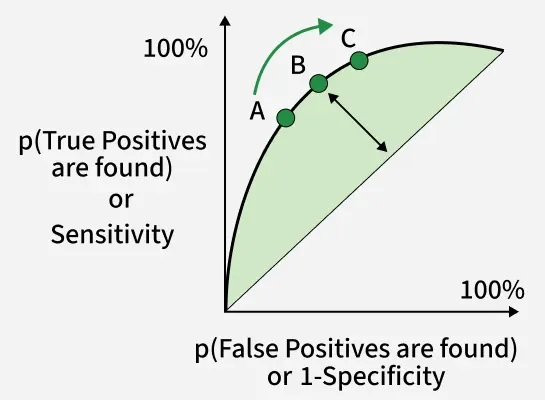
\includegraphics[width=0.7\textwidth]{roc_curve.png}
\caption{Sensitivity versus False Positive Rate plot (ROC Curve)}
\label{fig:roc_curve}
\end{figure}

These terms are derived from the confusion matrix which provides the following values:

\begin{itemize}
\item \textbf{True Positive (TP):} Correctly predicted positive instances
\item \textbf{True Negative (TN):} Correctly predicted negative instances
\item \textbf{False Positive (FP):} Incorrectly predicted as positive
\item \textbf{False Negative (FN):} Incorrectly predicted as negative
\end{itemize}

\begin{figure}[H]
\centering
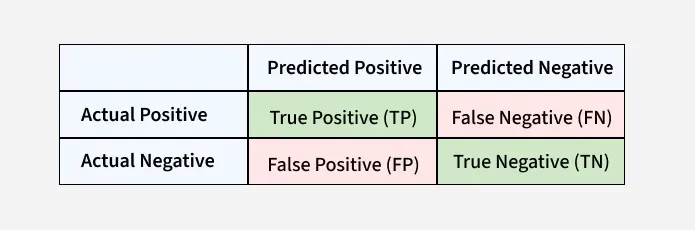
\includegraphics[width=0.6\textwidth]{confusion_matrix.png}
\caption{Confusion Matrix for a Classification Task}
\label{fig:confusion_matrix}
\end{figure}

\subsection{ROC Curve and AUC}

The ROC Curve plots TPR vs. FPR at different thresholds. It represents the trade-off between the sensitivity and specificity of a classifier.

\textbf{AUC (Area Under the Curve):} measures the area under the ROC curve. A higher AUC value indicates better model performance as it suggests a greater ability to distinguish between classes. An AUC value of 1.0 indicates perfect performance while 0.5 suggests it is random guessing.

\subsubsection{How AUC-ROC Works}

AUC-ROC curve helps us understand how well a classification model distinguishes between the two classes. Imagine we have 6 data points and out of these:
\begin{itemize}
\item 3 belong to the positive class: Class 1 for people who have a disease.
\item 3 belong to the negative class: Class 0 for people who don't have disease.
\end{itemize}

\subsubsection{When to Use AUC-ROC}

AUC-ROC is effective when:
\begin{itemize}
\item The dataset is balanced and the model needs to be evaluated across all thresholds.
\item False positives and false negatives are of similar importance.
\end{itemize}

\textbf{Model Performance with AUC-ROC:}
\begin{itemize}
\item \textbf{High AUC (close to 1):} The model effectively distinguishes between positive and negative instances.
\item \textbf{Low AUC (close to 0):} The model struggles to differentiate between the two classes.
\item \textbf{AUC around 0.5:} The model doesn't learn any meaningful patterns, i.e., it is doing random guessing.
\end{itemize}

\subsection{Precision and Recall Metrics}

\subsubsection{Precision}

It refers to the proportion of correct positive predictions (True Positives) out of all the positive predictions made by the model, i.e., True Positives + False Positives. It is a measure of the accuracy of the positive predictions. The formula for Precision is:

\begin{equation}
\text{Precision} = \frac{\text{True Positives}}{\text{True Positives} + \text{False Positives}}
\end{equation}

A high Precision means that the model makes few False Positives. This metric is especially useful when the cost of false positives is high, such as in email spam detection.

\subsubsection{Recall}

It is also known as Sensitivity or True Positive Rate, where we measure the proportion of actual positive instances that were correctly identified by the model. It is the ratio of True Positives to the total actual positives, i.e., True Positives + False Negatives. The formula for Recall is:

\begin{equation}
\text{Recall} = \frac{\text{True Positives}}{\text{True Positives} + \text{False Negatives}}
\end{equation}

A high Recall means the model correctly identifies most of the positive instances, which is critical when False Negatives are costly, like in medical diagnoses.

\subsubsection{Confusion Matrix}

To better understand Precision and Recall, we can use a Confusion Matrix which summarizes the performance of a classifier in four essential terms:

\begin{itemize}
\item \textbf{True Positives (TP):} Correctly predicted positive instances.
\item \textbf{False Positives (FP):} Incorrectly predicted positive instances.
\item \textbf{True Negatives (TN):} Correctly predicted negative instances.
\item \textbf{False Negatives (FN):} Incorrectly predicted negative instances.
\end{itemize}

\subsection{Precision-Recall Curve}

The Precision-Recall curve shows a comparison of sample PR and ROC curves. It is desired that the algorithm should have both high precision and high recall. However, most machine learning algorithms often involve a trade-off between the two. A good PR curve has greater AUC (area under the curve).

\begin{figure}[H]
\centering
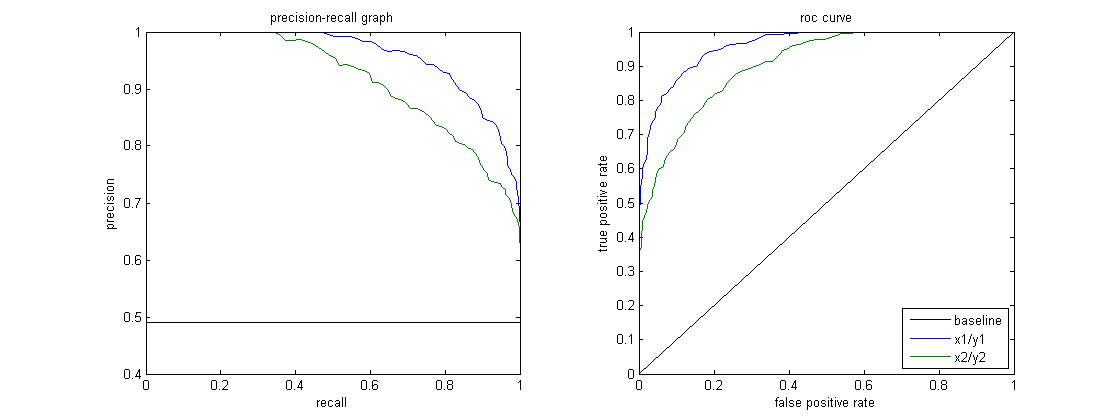
\includegraphics[width=0.8\textwidth]{pr_roc_fixed.png}
\caption{Comparison of Precision-Recall and ROC curves}
\label{fig:pr_roc}
\end{figure}

\subsubsection{When to Use PR Curve and ROC Curve}

Choosing between ROC and Precision-Recall depends on the specific needs of the problem, understanding data distribution, and the consequences of different types of errors.

The PR curve helps us visualize how well our model is performing across various thresholds. It provides insights into how changes in decision thresholds affect Precision and Recall. For example, increasing the threshold might increase Precision (i.e., fewer False Positives) but it could lower Recall (i.e., more False Negatives). The goal is to find a balance that best suits the specific needs of your application, whether it's minimizing False Positives or False Negatives.

ROC curves are suitable when the class distribution is balanced and false positives and false negatives have similar consequences. They show the trade-off between sensitivity and specificity.

\begin{figure}[H]
\centering
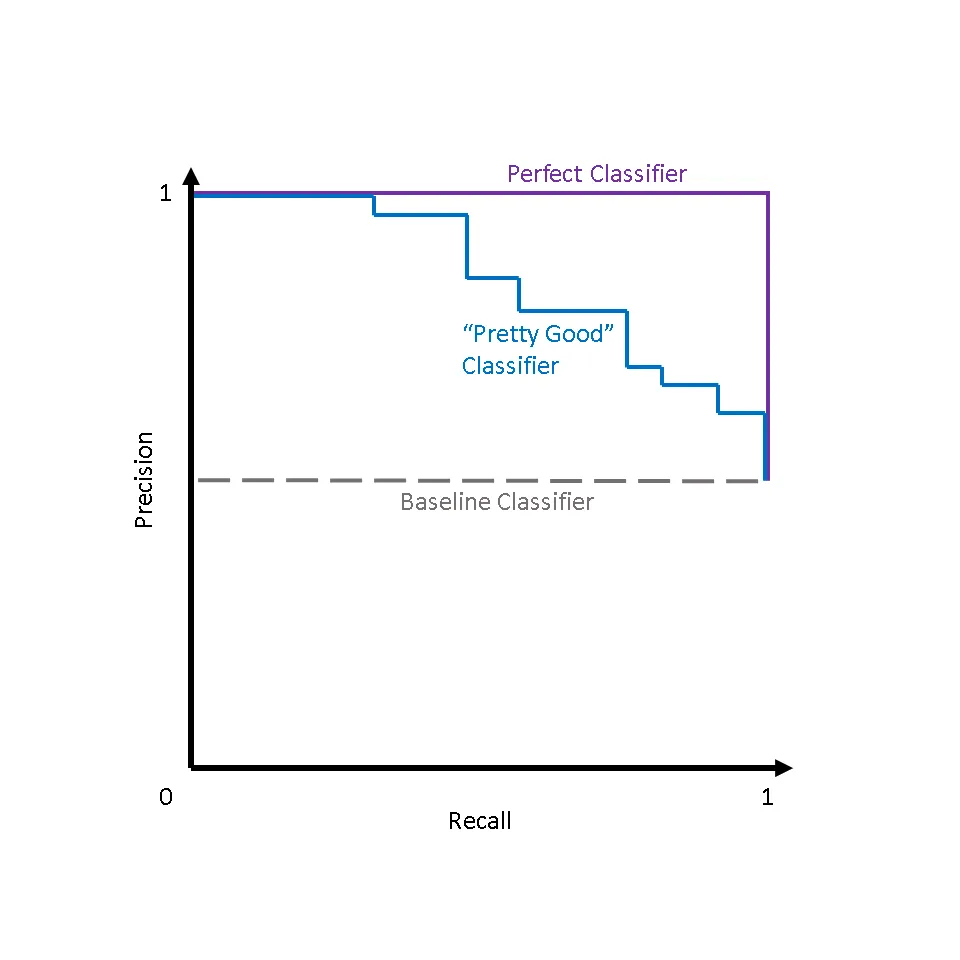
\includegraphics[width=0.8\textwidth]{precision_recall_comparison_fixed.png}
\caption{Precision-Recall comparison visualization}
\label{fig:precision_recall_comparison}
\end{figure}

The ideal is to construct a predicted group that includes all the minimum wage workers and none of the non-minimum wage workers, so both the precision and the recall are 1. Generally, the higher the precision for a given recall rate, the better the performance of the model is.

\section*{References}

CausalML\_book\_2022.pdf

\end{document}

